% Example LaTeX document for GP111 - note % sign indicates a comment
\documentclass[11pt]{article}

\usepackage{graphicx}
\usepackage{atbegshi,picture}
\usepackage{lipsum}
\usepackage{verbatim}

\usepackage{subcaption}
\usepackage{mwe}
\usepackage{hyperref}

\usepackage{textcomp}

\usepackage{array}
\newcolumntype{L}[1]{>{\raggedright\let\newline\\\arraybackslash\hspace{0pt}}m{#1}}




%--------------------------------VARS-----------------







%------ Copy Pasta from the webs logo

%----------------------------------------------------------------------------------------
%	TITLE PAGE
%----------------------------------------------------------------------------------------

\newcommand*{\titleGP}{\begingroup % Create the command for including the title page in the document
\centering % Center all text
\vspace*{\baselineskip} % White space at the top of the page
\begin{figure}[tbph]
\centering

\includegraphics[width=0.15\linewidth]{../media/logos/synercon_logo_v3_only}
\end{figure}
{\Huge \textbf{Forensic Link Adapter \\Quick Reference}}\\[2\baselineskip] % Title
{\Huge \textbf{CAT \\ADEM 3 \& ADEM4 \\[.4cm] ECMs}}\\[2\baselineskip] % Title
{\Huge Synercon Technologies LLC}\\[2\baselineskip]
{\Large For Software Version 1}\\[3cm]

\tableofcontents
\vfill % Whitespace between editor names and publisher logo


\textcopyright {\scshape 2015} \\[0.3\baselineskip] % Year
Synercon Technologies LLC

\endgroup}
%------ End copy pasta








% Default margins are too wide all the way around.  I reset them here
\setlength{\topmargin}{-.5in}
\setlength{\textheight}{9in}
\setlength{\oddsidemargin}{.125in}
\setlength{\textwidth}{6.25in}
\begin{document}
%\title{{\Huge Lease}}
%\author{ \\ \\ {\LARGE At Address  6772 E 26th Pl, Tulsa, OK 74129}
%Gavin Bauer\\
%(832) 630-9337
%}
%\renewcommand{\today}{June 11, 2013}
%\maketitle







\titleGP % This command includes the title page

\newpage
\section{About this document}
\paragraph{  }
This document is intended to be a quick guide to gathering data from CAT ADEM 3 and ADEM 4 ECMs. For a full explanation of the steps, or troubleshooting, please refer to the Field Guide or the User Manual.

\section{Downloading CAT ECMs}
\paragraph{  }
The FLA can extract standards-based data, such as vehicle miles, engine hours, and fault codes, as well as non-standards-based data, such as "Snapshot" and OEM History and Configuration data.
\paragraph{  }
To perform a download on a CAT ECM, plug the FLA into the diagnostic port, typically located on the driver's side, near the door and either under the dash, or by the seat. If the FLA does not power on, refer to the troubleshooting section of the Field Guide.
\\[\baselineskip]
\noindent\begin{minipage}{0.3\textwidth}% adapt widths of minipages to your needs
\begin{center}
\textbf{1}\\[\baselineskip]
\end{center}
Once the FLA finishes booting and reaches the title screen, begin the scan. If the Scan option is not avaliable, refer to the troubleshooting section of the Field Guide.
\end{minipage}%
\hfill%
\begin{minipage}{0.6\textwidth}
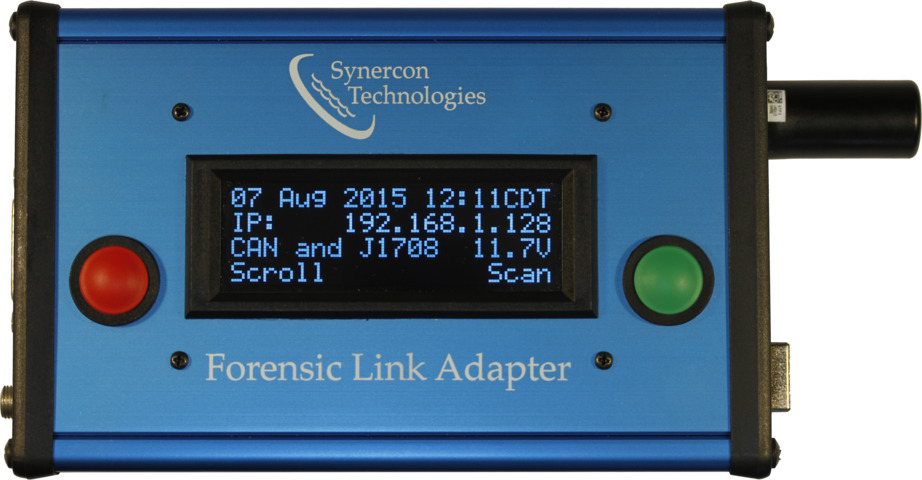
\includegraphics[width=\linewidth]{../media/fla_screens/ethernet_and_others/main/title_both}
\end{minipage}
\\[\baselineskip]
\noindent\begin{minipage}{0.3\textwidth}% adapt widths of minipages to your needs
\begin{center}
\textbf{2}\\[\baselineskip]
\end{center}
The FLA will first extract standards based data.
\end{minipage}%
\hfill%
\begin{minipage}{0.6\textwidth}
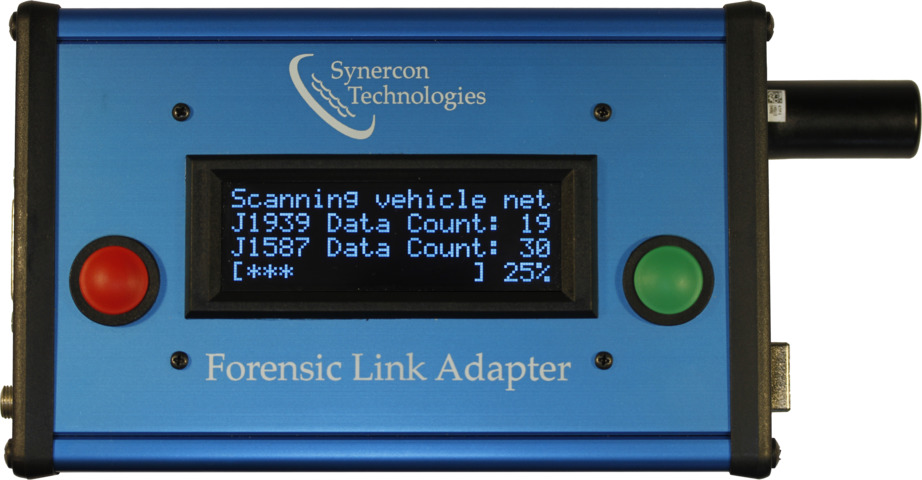
\includegraphics[width=\linewidth]{../media/fla_screens/ethernet_and_others/veh_scan/scan_25}
\end{minipage}
\\[\baselineskip]
\noindent\begin{minipage}{0.3\textwidth}% adapt widths of minipages to your needs
\begin{center}
\textbf{3}\\[\baselineskip]
\end{center}
The FLA will display the Component Id of the engine, as well as the first X characters of the VIN. The full VIN will be in the report. Selecting Continue (green button) will continue the scan, Back (red button) will cancel the scan.
\end{minipage}%
\hfill%
\begin{minipage}{0.6\textwidth}
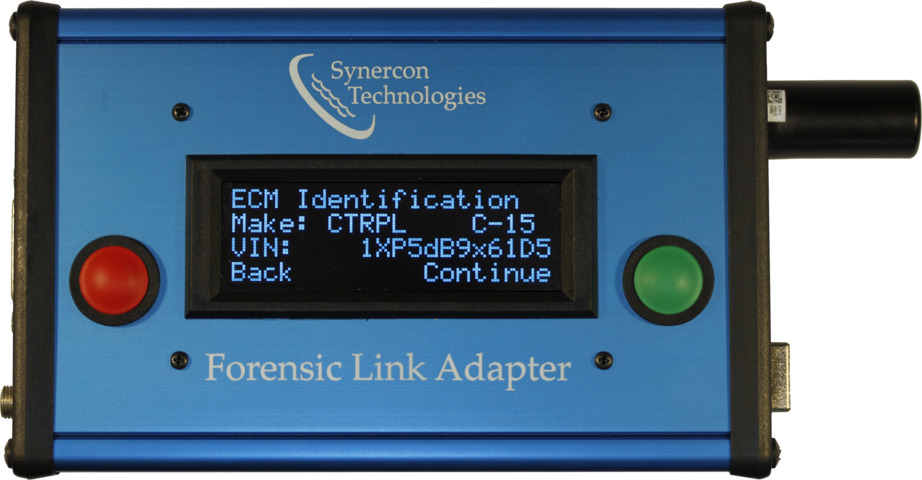
\includegraphics[width=\linewidth]{../media/fla_screens/ethernet_and_others/veh_scan/comp_id}
\end{minipage}
\\[\baselineskip]
\noindent\begin{minipage}{0.3\textwidth}% adapt widths of minipages to your needs
\begin{center}
\textbf{4}\\[\baselineskip]
\end{center}
This screen will ask if the user wishes to collect non-standards based data. If the ECM is not supported, ensure the ECM is in the list of supported ECMs. Select Get Data.
\end{minipage}%
\hfill%
\begin{minipage}{0.6\textwidth}
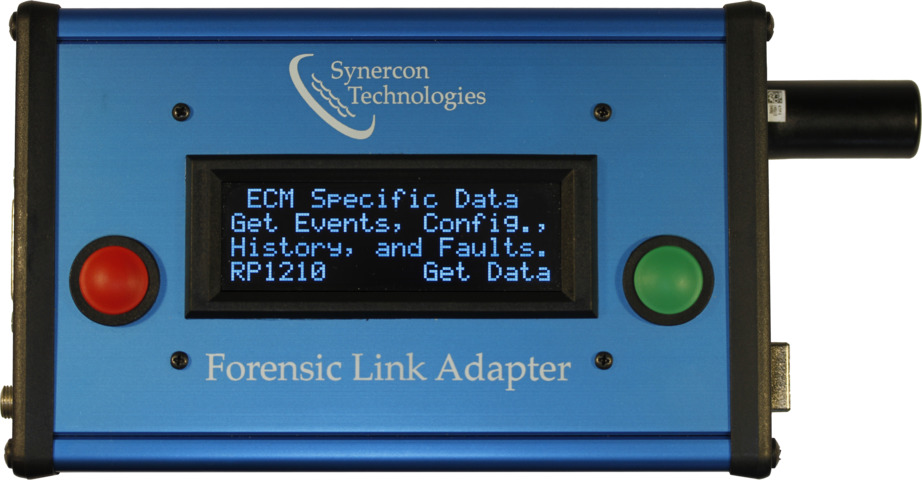
\includegraphics[width=\linewidth]{../media/fla_screens/ethernet_and_others/veh_scan/get_ecm_specific}
\end{minipage}
\\[\baselineskip]
\noindent\begin{minipage}{0.3\textwidth}% adapt widths of minipages to your needs
\begin{center}
\textbf{5}\\[\baselineskip]
\end{center}
The FLA will begin collecting Configuration, Historical, Live, and Snapshot data from the ECM.
\end{minipage}%
\hfill%
\begin{minipage}{0.6\textwidth}
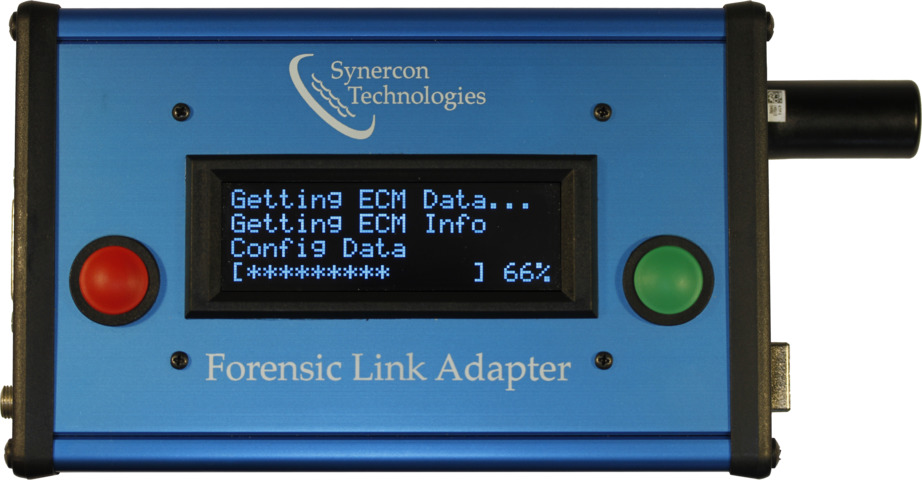
\includegraphics[width=\linewidth]{../media/fla_screens/ethernet_and_others/veh_scan/ecm_config}
\end{minipage}
\\[\baselineskip]
\noindent\begin{minipage}{0.3\textwidth}% adapt widths of minipages to your needs
\begin{center}
\textbf{6}\\[\baselineskip]
\end{center}
After complete, the operator will be asked if they wish to enter RP1210 mode, or proceed to the upload screen. Unless the operator wishes to collect data using OEM software, proceed to the upload screen.
\end{minipage}%
\hfill%
\begin{minipage}{0.6\textwidth}
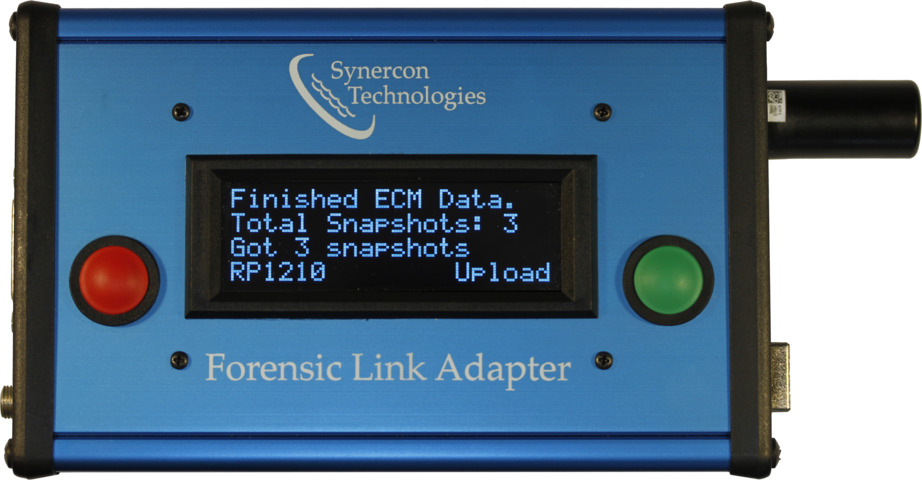
\includegraphics[width=\linewidth]{../media/fla_screens/ethernet_and_others/veh_scan/ecm_finished}
\end{minipage}\\[\baselineskip]
The download is now complete, and the data package can be previewed on the FLA Preview.
\paragraph{  }
If the download was performed in the field, the operator can enable the DHCP service, and connect a computer to the FLA using the Ethernet cable in the FLA case. Your computer should detect a network with no Internet connection.
\paragraph{  }
If the download was performed in a location that has a working Ethernet jack, such as a bench download at a office, the user can upload the data immediately, and examine the full report on the FLA Portal.

\section{Verifying Data in the Field}
\paragraph{  }
The FLA is able to give the user an overview of the data in the field through the FLA Preview. The FLA Preview is a website hosted by the FLA that allows the user to connect to the device and examine data on it.
\subsection{Accessing the FLA Preview in the field}
To access the FLA Preview without an Internet connection, follow these steps.\\[\baselineskip]
\noindent\begin{minipage}{0.3\textwidth}% adapt widths of minipages to your needs
\begin{center}
\textbf{1}\\[\baselineskip]
\end{center}
Power on the FLA. If no download is in progress, the FLA does not need to be connected to the vehicle via the diagnostic cable, the cigarette lighter adapter can be used.
\end{minipage}%
\hfill%
\begin{minipage}{0.6\textwidth}
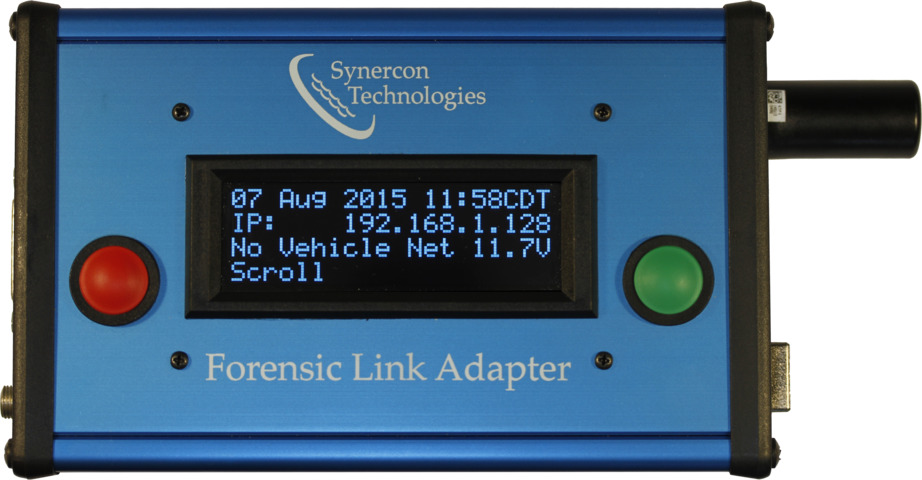
\includegraphics[width=\linewidth]{../media/fla_screens/ethernet_and_others/main/title_no_net}
\end{minipage}\\[\baselineskip]
\noindent\begin{minipage}{0.3\textwidth}% adapt widths of minipages to your needs
\begin{center}
\textbf{2}\\[\baselineskip]
\end{center}
Enable the DHCP services on the FLA. For more information on how to enable DHCP services, refer to the Field Guide. Verify the services are on by confirming the IP address of the device is 10.0.0.1
\end{minipage}%
\hfill%
\begin{minipage}{0.6\textwidth}
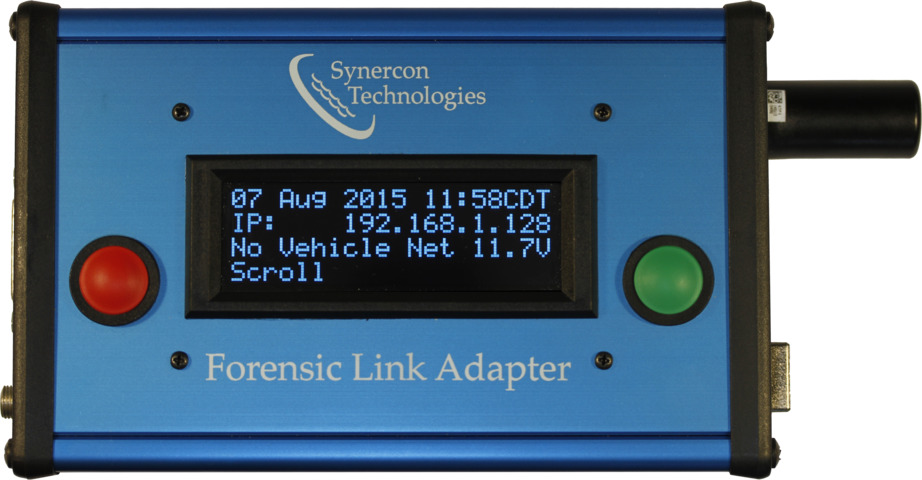
\includegraphics[width=\linewidth]{../media/fla_screens/ethernet_and_others/main/title_no_net}
\end{minipage}\\[\baselineskip]
\noindent\begin{minipage}{0.3\textwidth}% adapt widths of minipages to your needs
\begin{center}
\textbf{3}\\[\baselineskip]
\end{center}
Connect the computer to the FLA via the included Ethernet cable.
\end{minipage}%
\hfill%
\begin{minipage}{0.6\textwidth}
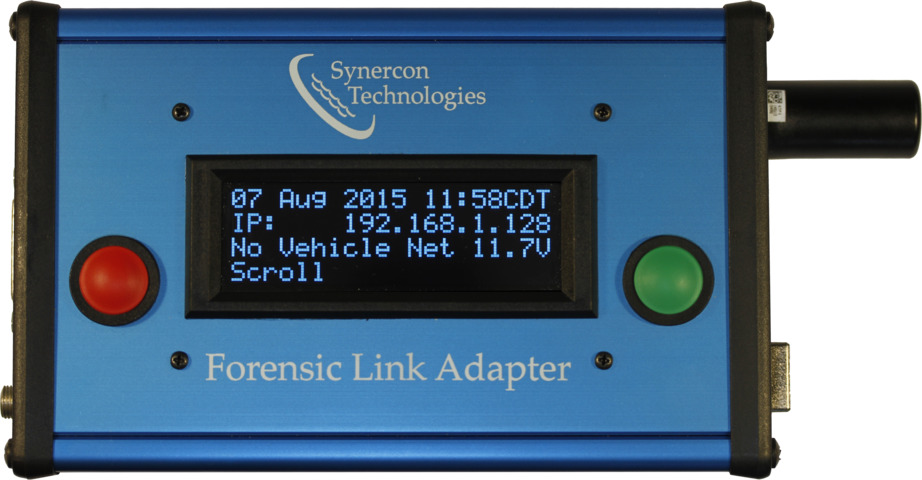
\includegraphics[width=\linewidth]{../media/fla_screens/ethernet_and_others/main/title_no_net}
\end{minipage}\\[\baselineskip]
\noindent\begin{minipage}{0.3\textwidth}% adapt widths of minipages to your needs
\begin{center}
\textbf{4}\\[\baselineskip]
\end{center}
On the computer connected to the FLA, type the following in to the address bar exactly:\\
10.0.0.1
\end{minipage}%
\hfill%
\begin{minipage}{0.6\textwidth}
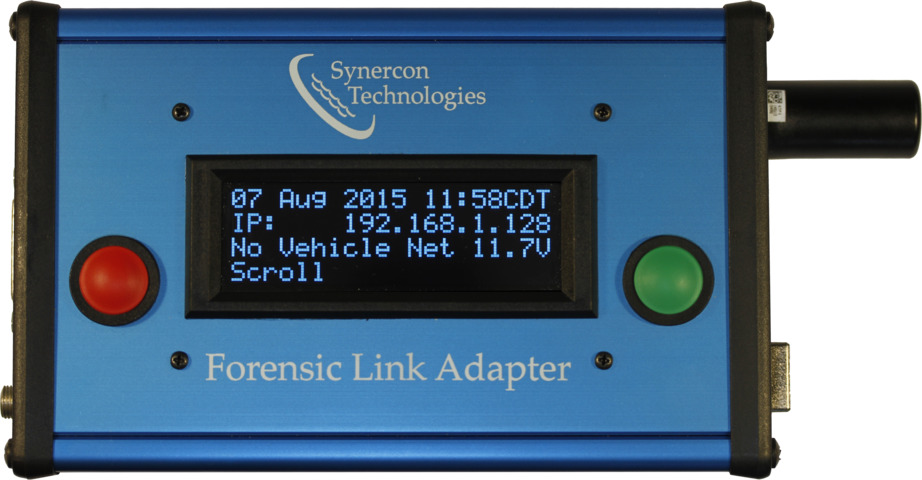
\includegraphics[width=\linewidth]{../media/fla_screens/ethernet_and_others/main/title_no_net}
\end{minipage}\\[\baselineskip]
If the FLA Preview website does not load after these steps, refer to the troubleshooting part of the Field Guide.
\subsection{Accessing the FLA Preview in the office, or at home}
\noindent\begin{minipage}{0.3\textwidth}% adapt widths of minipages to your needs
\begin{center}
\textbf{1}\\[\baselineskip]
\end{center}
Verify the DHCP services are off by examining the IP address of the title screen. If the address is 10.0.0.1 the DHCP services are on and need to be disabled.
\end{minipage}%
\hfill%
\begin{minipage}{0.6\textwidth}
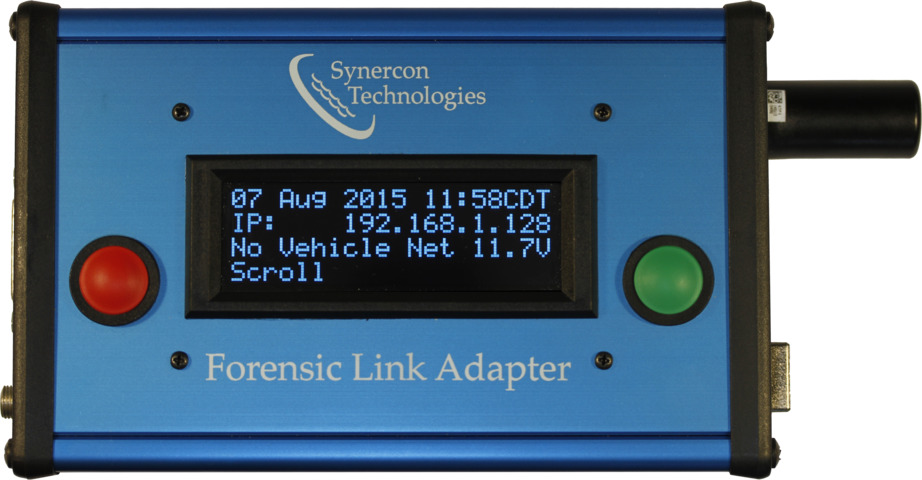
\includegraphics[width=\linewidth]{../media/fla_screens/ethernet_and_others/main/title_no_net}
\end{minipage}\\[\baselineskip]
\noindent\begin{minipage}{0.3\textwidth}% adapt widths of minipages to your needs
\begin{center}
\textbf{2}\\[\baselineskip]
\end{center}
Plug the FLA into a known working Ethernet port. The FLA should find an IP address and display it on the title screen.
\end{minipage}%
\hfill%
\begin{minipage}{0.6\textwidth}
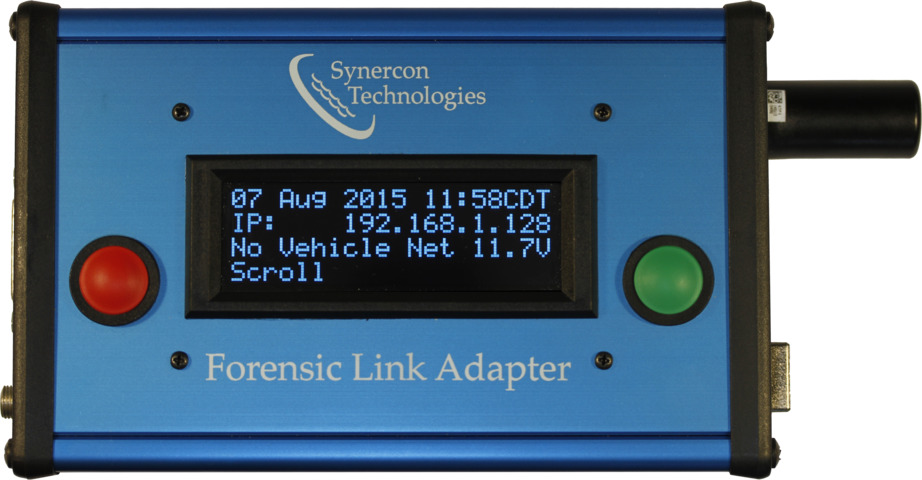
\includegraphics[width=\linewidth]{../media/fla_screens/ethernet_and_others/main/title_no_net}
\end{minipage}\\[\baselineskip]
\noindent\begin{minipage}{0.3\textwidth}% adapt widths of minipages to your needs
\begin{center}
\textbf{3}\\[\baselineskip]
\end{center}
Enter this address into the address bar of a web browser of a computer connected to the same network. If the FLA Preview site does not load, refer to the troubleshooting section of the Field Guide.
\end{minipage}%
\hfill%
\begin{minipage}{0.6\textwidth}
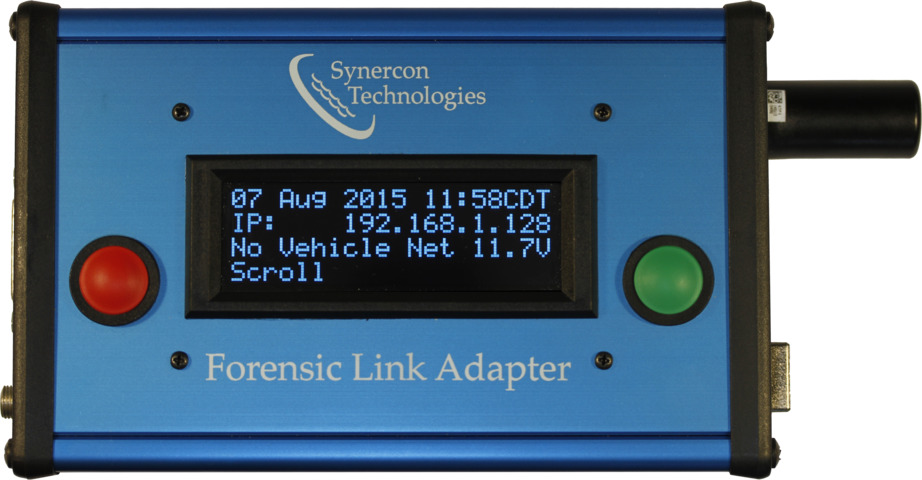
\includegraphics[width=\linewidth]{../media/fla_screens/ethernet_and_others/main/title_no_net}
\end{minipage}\\[\baselineskip]
\subsection{The FLA Preview Website}
\paragraph{}
The main page of the FLA will show the user how many pending data packages there are on the FLA, as well as if there are any downloads in progress.
\begin{figure}[tbph]
\centering
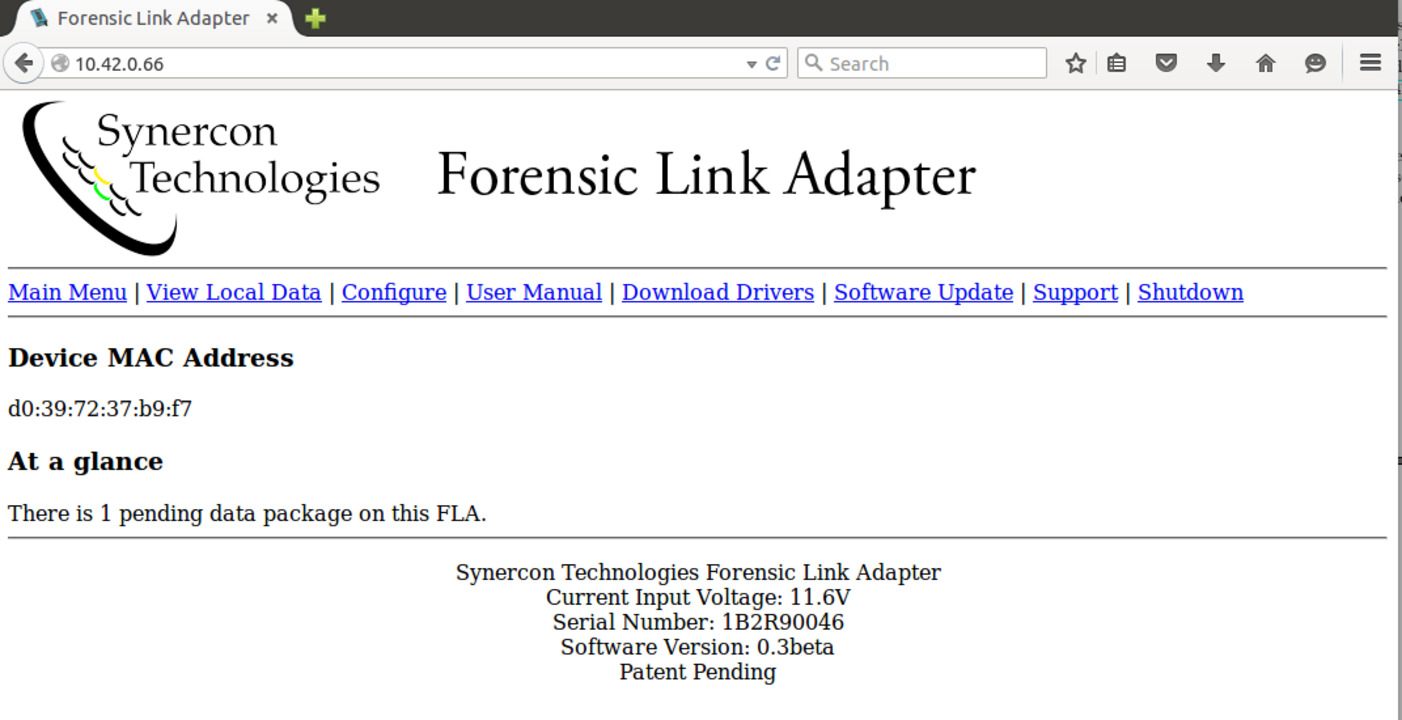
\includegraphics[width=.95\linewidth]{../media/fla_preview_screenshots/main_page}
\label{fig:fla_preview_main_page}
\end{figure}
\paragraph{  }
Navigating to the View Local Data page gives a brief overview of each data package on the FLA that is not yet uploaded. The OEM data column indicates if the FLA has extracted data from the engine that is not a part of the standards-based extraction. From this page the operator can view the data from an individual data, view archived data packages, or archive pending data packages.
\begin{figure}[tbph]
\centering
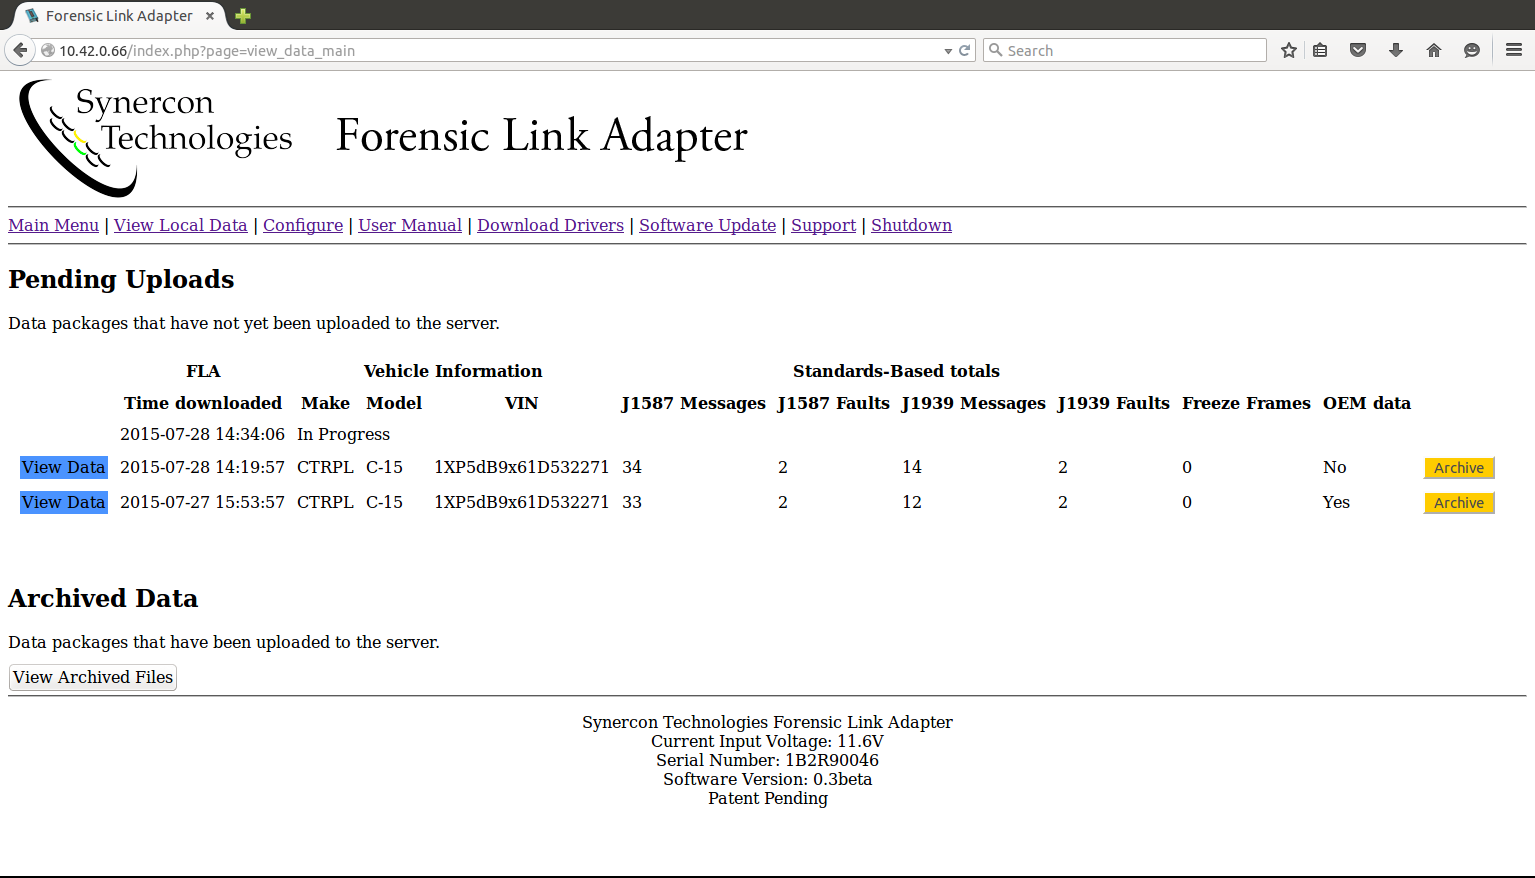
\includegraphics[width=.95\linewidth]{../media/fla_preview_screenshots/local_data}
\label{fig:fla_preview_local_data}
\end{figure}
\paragraph{  }
Archiving a pending data package will move the data package to the archived list, and it will NOT be uploaded to the server. For more information about archiving a pending data package, refer to the Field Guide.
\paragraph{  }
The View Data button will allow the operator to view a preview of the report. This will contain all of the standards-based messages, as well as standards-based faults. For CAT ECMs, an abbreviated part of the avaliable Quick-Stop, Diagnostic, and External Trigger Snapshots. The full records will be avaliable once the operator uploads the data to the Synercon Portal. When viewing the report, there will be buttons to download the avaliable snapshots at the top of the report, as shown below.
\begin{figure}[tbph]
\centering
% 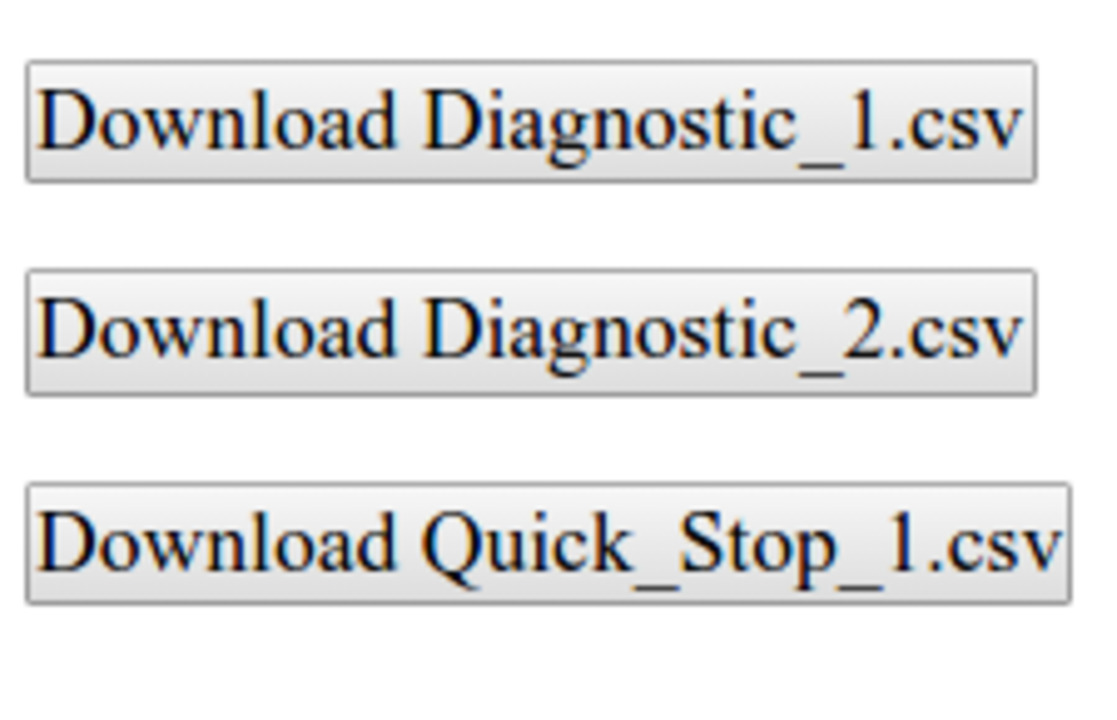
\includegraphics[width=.3\linewidth]{../media/fla_preview_screenshots/csv_download}
\end{figure}

\paragraph{  }
The data in the FLA Preview is intended to be a summary of the information gathered by the FLA. A full report is only avaliable once the user uploads the report to the FLA Portal. For more information about the FLA Preview, or uploading data, refer to the Field Guide.


\end{document}
